\documentclass{standalone}
\usepackage{amsmath}
\usepackage{tikz}

\begin{document}
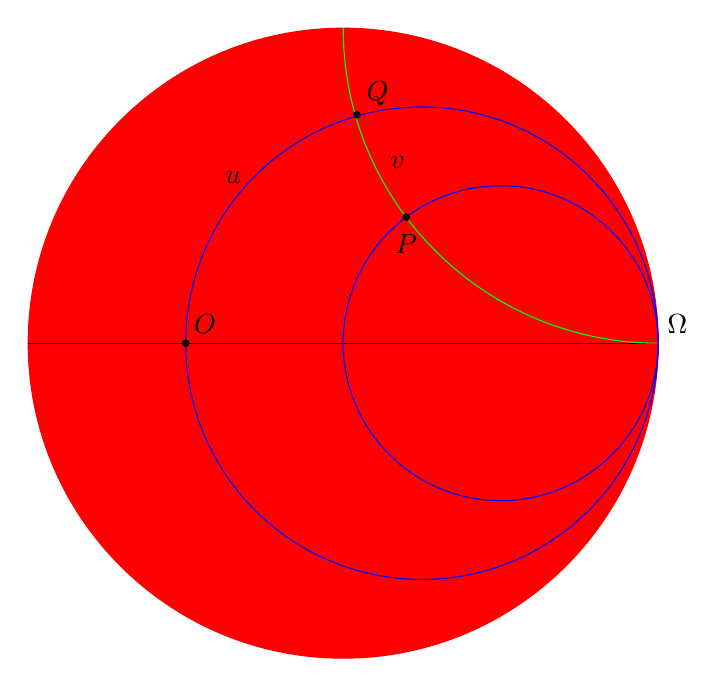
\begin{tikzpicture}
    \node[anchor=225] at (4,2) {$\Omega$};
    \draw[red,fill=red] (0,2) circle[radius=4];
    \draw[blue] (1, 2) circle[radius=3];
    \draw[black] (-4,2) -- (4,2);
    \draw[green] (4,2) arc (-90:-180:4);
    \draw[blue] (2, 2) circle[radius=2];
    \node[fill,circle,inner sep=1pt] at (-2,2) {};
    \node[anchor=225] at (-2,2) {$O$};
    \node[fill,circle,inner sep=1pt] at (0.175,4.9) {};
    \node[anchor=225] at (0.175,4.9) {$Q$};
    \node[fill,circle,inner sep=1pt] at (0.8,3.6) {};
    \node[anchor=90] at (0.8,3.5) {$P$};
    \node[anchor=225] at (0.49,4.1) {$v$};
    \node[anchor=225] at (-1.6,3.9) {$u$};
\end{tikzpicture}
\end{document}
